
\chapter{Problems in three dimensions}

For three dimensional equations, the domain of the system $\Omega \in \R^3$ and Sobolev space (\ref{sobolev_space}) becomes
\begin{align}
  \label{3d_sobolev_space}
  \mathcal{H}^1(\Omega) &= \left\{ u\ :\ \Omega \rightarrow \R\ \Bigg|\ u, \parder{u}{x}, \parder{u}{y}, \parder{u}{z} \in L^2(\Omega) \right\},
\end{align}
and the domain is discretized into either tetrahedral or brick elements, with new interpolation functions that satisfy 3D interpolation properties analogous to (\ref{interpolation_properties}).  For an excellent explanation of the resulting 3D Galerkin system analogous to (\ref{intro_galerkin_system}), see \citet{elman_2005}.

In this chapter, we solve the three-dimensional variant of heat equation (\ref{intro_ode}) and the Stokes equations.

%===============================================================================

\section{Poisson equation}

\index{Linear differential equations!3D}
\index{Poisson equation}
The Poisson equation to be solved over the domain $\Omega = [-\pi,\pi] \times [-\pi,\pi] \times [-\pi,\pi]$ is
\begin{align}
  \label{3d_poisson_start}
  -\nabla^2 u &= f &&\text{ in } \Omega \\
  f &= 10 \exp\left( -\frac{x^2}{2} - \frac{y^2}{2} - \frac{z^2}{2}\right) &&\text{ in } \Omega \\
  \nabla u \cdot \normal &= g_{N_y} = \sin(x) &&\text{ on } \Gamma_N, \Gamma_S \\
  \nabla u \cdot \normal &= g_{N_x} = 0 &&\text{ on } \Gamma_E, \Gamma_W \\
  \label{3d_poisson_end}
  u &= g_D = 0 &&\text{ on } \Gamma_T, \Gamma_B,
\end{align}
where $\Gamma_N$, $\Gamma_S$, $\Gamma_E$, and $\Gamma_W$ are the North, South, East and West boundaries, $\Gamma_T$ and $\Gamma_B$ are the top and bottom boundaries, and $\normal$ is the outward unit normal to the boundary $\Gamma$.

The associated Galerkin weak form with test function $\phi \in \testspace$ defined by (\ref{test_space}) is
{\footnotesize
\begin{align*}
  -\int_{\Omega} \nabla^2 u \phi \d{\Omega} &= \int_{\Omega} f \phi \d{\Omega} \\
  \int_{\Omega} \nabla u \cdot \nabla \phi \d{\Omega} - \int_{\Gamma} \phi \nabla u \cdot \normal \d{\Gamma} &= \int_{\Omega} f \phi \d{\Omega} \\
  \int_{\Omega} \nabla u \cdot \nabla \phi \d{\Omega} - \int_{\Gamma_N} \phi g_{N_y} \d{\Gamma_N} - \int_{\Gamma_S} \phi g_{N_y} \d{\Gamma_S} &= \int_{\Omega} f \phi \d{\Omega},
\end{align*}}
and so the discrete variational problem consists of finding $u \in \trialspace$ given by (\ref{trial_space}) such that
\begin{align*}
  a(u,\phi) &= l(\phi) && \forall \phi \in S_0^h \subset \mathcal{H}_{E_0}^1(\Omega),
\end{align*}
subject to Dirichlet condition (\ref{3d_poisson_end}), where
\begin{align*}
  l(\phi) &= \int_{\Gamma_N} \phi g_{N_y} \d{\Gamma_N} + \int_{\Gamma_S} \phi g_{N_y} \d{\Gamma_S} + \int_{\Omega} f \phi \d{\Omega}, \\
  a(u,\phi) &= \int_{\Omega} \nabla u \cdot \nabla \phi \d{\Omega}.
\end{align*}
This is as far as is needed to proceed in order to solve this simple problem with FEniCS, as demonstrated by Code Listing \ref{3d_poisson_code} and Figures \ref{3d_poisson_image_1} and \ref{3d_poisson_image_2}.

\pythonexternal[label=3d_poisson_code, caption={FEniCS code used to solve 3D-Poisson problem (\ref{3d_poisson_start} -- \ref{3d_poisson_end}).}]{scripts/fenics_intro/3D_poisson.py}
  
\begin{figure}
  \centering
    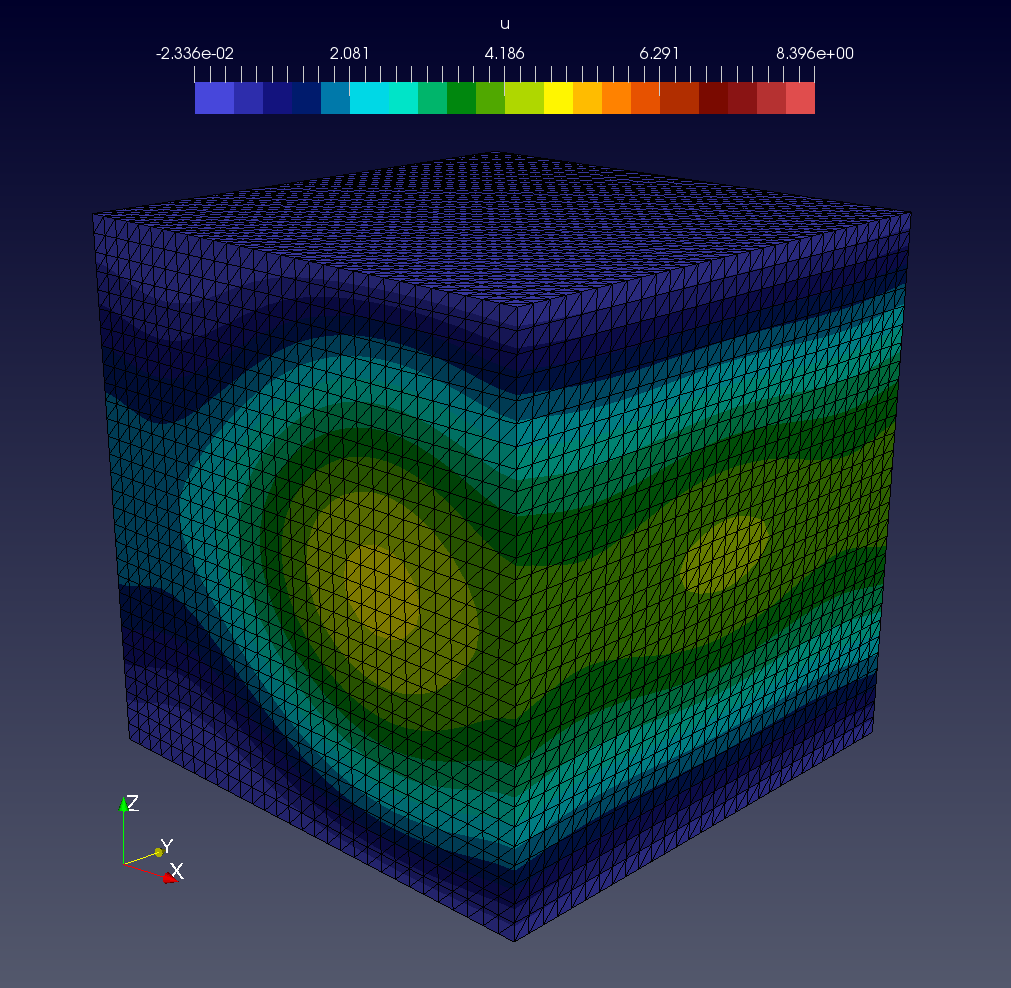
\includegraphics[width=\linewidth]{images/fenics_intro/3Dpoisson_new.png}
  \caption[Three-dimensional Poisson solution]{Poisson equation solution to (\ref{3d_poisson_start} -- \ref{3d_poisson_end}) defined over a $30 \times 30 \times 30$ element mesh.}
  \label{3d_poisson_image_1}
\end{figure}

\begin{figure}
  \centering
    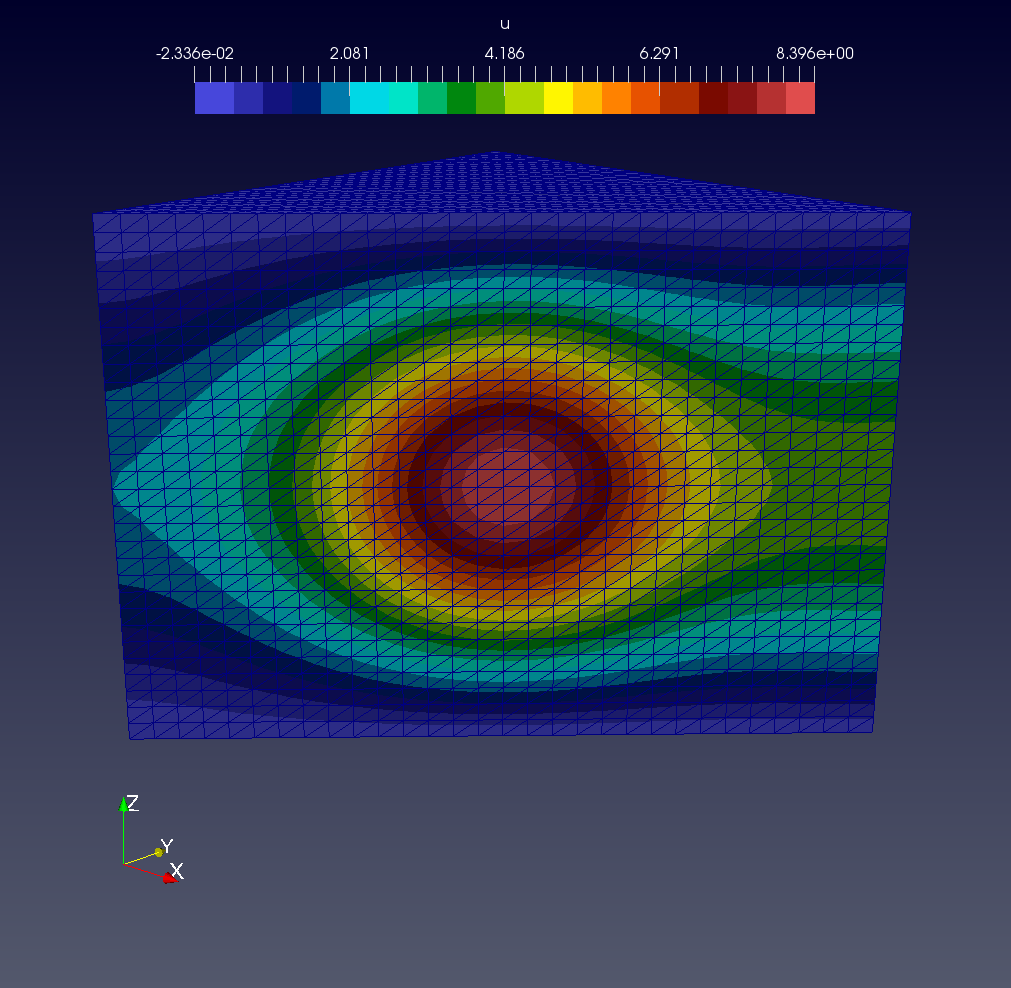
\includegraphics[width=\linewidth]{images/fenics_intro/3Dpoisson_new_split.png}
  \caption[Inside the three-dimensional Poisson solution]{Inside the Poisson solution represented by Figure \ref{3d_poisson_image_1}.}
  \label{3d_poisson_image_2}
\end{figure}

%===============================================================================

\section{Stokes equations} \label{ssn_intro_stokes_3d}

\index{Linear differential equations!3D}
\index{Stokes equations!No-slip}
Recall from \S \ref{ssn_intro_stokes_2d} that the Stokes equations for an incompressible fluid are
\begin{align}
  \label{intro_stokes_3d_momentum}
  -\nabla \cdot \ranktwo{\sigma} &= \rankone{f} &&\text{ in } \Omega &&\leftarrow \text{ conservation of momentum} \\
  \label{intro_stokes_3d_mass}
  \nabla \cdot \rankone{u} &= 0 &&\text{ in } \Omega &&\leftarrow \text{ conservation of mass},
\end{align}
where $\ranktwo{\sigma}$ is the Cauchy-stress tensor defined as $\ranktwo{\sigma} = 2\eta \ranktwo{\dot{\epsilon}} - p\ranktwo{I}$; viscosity $\eta$, strain-rate tensor
\begin{align}
  \label{intro_strain_rate_tensor}
  \ranktwo{\dot{\epsilon}} &= \frac{1}{2}\left[\nabla \rankone{u} + (\nabla \rankone{u})\T \right] \notag \\
  &= \begin{bmatrix}
       \parder{u}{x} & \frac{1}{2}\left( \parder{u}{y} + \parder{v}{x} \right) & \frac{1}{2}\left( \parder{u}{z} + \parder{w}{x} \right) \\
       \frac{1}{2}\left( \parder{v}{x} + \parder{u}{y} \right) & \parder{v}{y} & \frac{1}{2}\left( \parder{v}{z} + \parder{w}{y} \right) \\
       \frac{1}{2}\left( \parder{w}{x} + \parder{u}{z} \right) & \frac{1}{2}\left( \parder{w}{y} + \parder{v}{z} \right) & \parder{w}{z}
     \end{bmatrix},
\end{align}
velocity $\rankone{u} = [u\ v\ w]\T$ with components $u$, $v$, $w$ in the $x$, $y$, and $z$ directions, and pressure $p$; and vector of internal forces $\rankone{f} = \rho \rankone{g}$ composed of material density $\rho$ and gravitational acceleration vector $\rankone{g} = [0\ 0\ \text{-}g]\T$.  For our example we use boundary conditions
\begin{align}
  \label{intro_stokes_3d_bc_n}
  \ranktwo{\sigma} \cdot \normal &= \rankone{g_N} = \rankone{0} &&\text{ on } \Gamma_T, \Gamma_B \\
  \label{intro_stokes_3d_bc_d}
  \rankone{u} &= \rankone{g_D} = \rankone{0} && \text{ on } \Gamma_L,
\end{align}
where $\Gamma_T$, $\Gamma_B$, and $\Gamma_L$ are the top, bottom, and lateral boundaries and $\normal$ is the outward-pointing normal vector.

It may be of interest to see how the conservation of momentum equations look in their expanded form,
\begin{align*}
  -\nabla \cdot \ranktwo{\sigma} &= \rankone{f} \\
  \begin{bmatrix}
    \parder{\sigma_{xx}}{x} + \parder{\sigma_{xy}}{y} + \parder{\sigma_{xz}}{z} \\ 
    \parder{\sigma_{yx}}{x} + \parder{\sigma_{yy}}{y} + \parder{\sigma_{yz}}{z} \\ 
    \parder{\sigma_{zx}}{x} + \parder{\sigma_{zy}}{y} + \parder{\sigma_{zz}}{z} \\ 
  \end{bmatrix} &=
  \begin{bmatrix}
    0 \\ 0 \\ \rho g
  \end{bmatrix}
\end{align*}
so that we have three equations,
{\tiny
\begin{subequations}
  \label{3d_stokes_expanded}
  \begin{eqnarray}
  \parder{}{x} \left[2\eta \parder{u}{x} \right]  - \parder{p}{x} + \parder{}{y} \left[\eta \left( \parder{u}{x} + \parder{v}{y} \right) \right] + \parder{}{z} \left[\eta \left( \parder{u}{x} + \parder{w}{z} \right) \right] &= 0 \\ 
  \parder{}{x} \left[\eta \left( \parder{v}{y} + \parder{u}{x} \right) \right]  + \parder{}{y} \left[2\eta \parder{v}{y} \right] - \parder{p}{y} + \parder{}{z} \left[\eta \left( \parder{v}{y} + \parder{w}{z} \right) \right] &= 0 \\ 
  \parder{}{x} \left[\eta \left( \parder{w}{z} + \parder{u}{x} \right) \right]  + \parder{}{y} \left[\eta \left( \parder{w}{z} + \parder{v}{y} \right) \right] + \parder{}{z} \left[2\eta \parder{w}{z} \right] - \parder{p}{z} &= \rho g,
  \end{eqnarray}
\end{subequations}}
which when combined with conservation-of-mass (\ref{intro_stokes_3d_mass}),
\begin{align*}
  \nabla \cdot \rankone{u} &= \parder{u}{x} + \parder{v}{y} + \parder{w}{z} = 0, 
\end{align*}
gives four equations and four unknowns $u$, $v$, $w$, and $p$.

The weak form for this problem is formed by taking the inner product of both sides of conservation of momentum equation (\ref{intro_stokes_3d_momentum}) with the vector test function $\rankone{\Phi} = [\phi\ \psi\ \chi]\T \in \rankone{S_0^h} \subset \left( \mathcal{H}_{E_0}^1(\Omega) \right)^3$ (see test space (\ref{test_space})) integrating over the domain $\Omega$,
\begin{align*}
  -\int_{\Omega} \nabla \cdot \ranktwo{\sigma} \cdot \rankone{\Phi} \d{\Omega} &= \int_{\Omega} \rankone{f} \cdot \rankone{\Phi} \d{\Omega},
\end{align*}
then integrate by parts to get 
\begin{align*}
  \int_{\Omega} \ranktwo{\sigma} : \nabla \rankone{\Phi} \d{\Omega} - \int_{\Gamma} \ranktwo{\sigma} \cdot \normal \cdot \rankone{\Phi} \d{\Gamma} &= \int_{\Omega} \rankone{f} \cdot \rankone{\Phi} \d{\Omega} \\
  \int_{\Omega} \ranktwo{\sigma} : \nabla \rankone{\Phi} \d{\Omega} &= \int_{\Omega} \rankone{f} \cdot \rankone{\Phi} \d{\Omega},
\end{align*}
where the fact that all boundaries are either homogeneous Neumann or Dirichlet has been used to eliminate boundary integrals.  Next, multiplying incompressibility (conservation of mass) equation (\ref{intro_stokes_3d_mass}) by the test function $\xi \in M^h \subset L^2(\Omega)$ (see $L^2$ space (\ref{l2_space})) also integrating over $\Omega$,
\begin{align*}
  \int_{\Omega} \left( \nabla \cdot \rankone{u} \right) \xi \d{\Omega} &= 0.
\end{align*}

Finally, using the fact that the right-hand side of incompressibility equation (\ref{intro_stokes_3d_mass}) is zero, the mixed formulation \index{Mixed methods} consists of finding mixed approximation $\rankone{u} \in \rankone{S_E^h} \subset \left( \mathcal{H}_E^1(\Omega) \right)^3$ (see trial space (\ref{trial_space})) and $p \in M^h \subset L^2(\Omega)$ such that
{\footnotesize
\begin{align}
  \label{intro_stokes_3d_mixed_problem}
  a(\rankone{u},p,\rankone{\Phi},\xi) &= L(\rankone{\Phi}) && \forall \rankone{\phi} \in \rankone{S_0^h} \subset \left( \mathcal{H}_{E_0}^1(\Omega) \right)^3,\ \xi \in M^h \subset L^2(\Omega),
\end{align}}
subject to Dirichlet condition (\ref{intro_stokes_3d_bc_d}) and
\begin{align*}
  a(\rankone{u},p,\rankone{\Phi},\xi) &= \int_{\Omega} \ranktwo{\sigma} : \nabla \rankone{\Phi} \d{\Omega} + \int_{\Omega} \left( \nabla \cdot \rankone{u} \right) \xi \d{\Omega}, \\
  L(\rankone{\Phi}) &= \int_{\Omega} \rankone{f} \cdot \rankone{\Phi} \d{\Omega}.
\end{align*}

For our solution satisfying inf-sup condition (\ref{inf_sup_condition}), we enrich the finite element space with bubble functions (see Chapter \ref{ssn_subgrid_scale_effects}), thus creating MINI elements \citep{arnold_1984}.  The solution is generated with Code Listing \ref{intro_3d_stokes_code} and depicted in Figure \ref{intro_3d_stokes_image}.

\pythonexternal[label=intro_3d_stokes_code, caption={FEniCS solution to 3D-Stokes-no-slip problem (\ref{intro_stokes_3d_mixed_problem}).}]{scripts/fenics_intro/3D_stokes.py}

\begin{figure*}
  \centering
    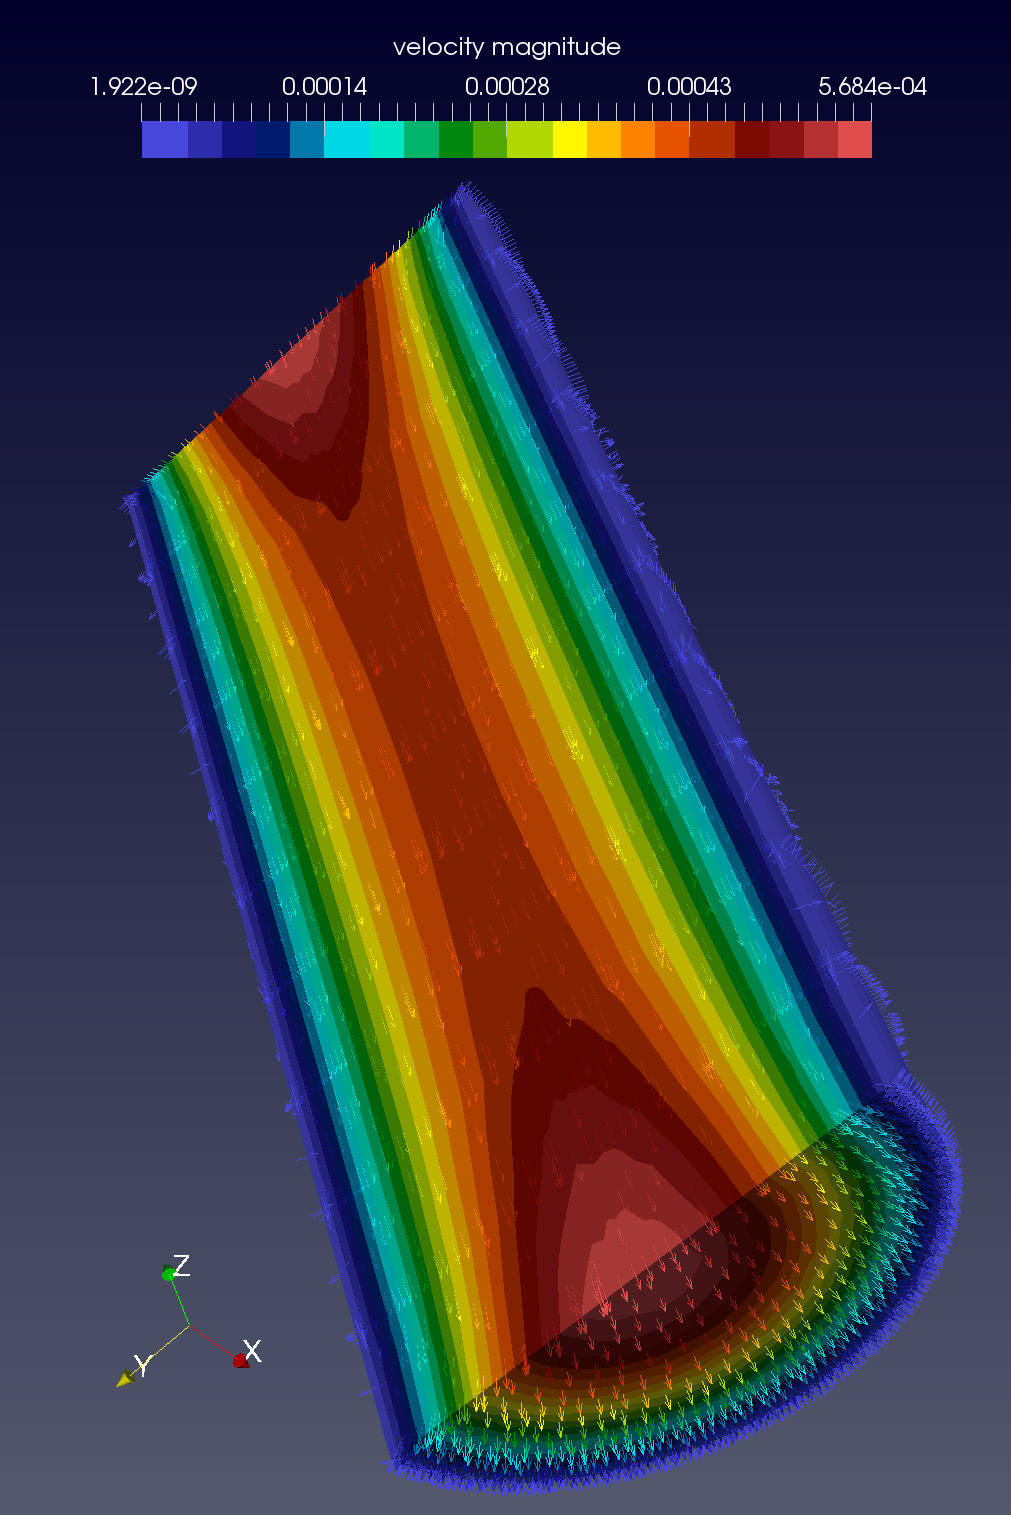
\includegraphics[width=0.8\linewidth]{images/fenics_intro/3Dstokes_new.png}
  \caption[Three-dimensional-no-slip Stokes example]{Inside Stokes velocity solution $\rankone{u}$ in m s\sups{-1} within a tube of diameter 1 mm and height 5 mm filled with honey at density $\rho = 1420$ kg m$^{-3}$ and viscosity $\eta = 8$ Pa s.  Gravity forces the honey in the $-z$ direction, as indicated by the overlain velocity vectors.}
  \label{intro_3d_stokes_image}
\end{figure*}
